\section{Overview} % (fold)
\label{sec:overview}
    
    Per il seguente progetto si è scelto di analizzare il famoso puzzle/problema di ottimizzazione chiamato \emph{Eternity 2}, attraverso euristiche basate su ricerca locale.

    Nel seguito, indicheremo con il termine \textit{tile} una cella della \textit{board} di gioco; inoltre, dato che ogni tile ha un quattro possibili orientamenti, questi ultimi verranno indicati con i numeri $0$, $1$, $2$ e $3$, dove $0$ è l'orientamento originale (cioè quello letto dal file di input) ed $i \in \{1,2,3\}$ è l'orientamento ottenuto ruotando di $i*90$ gradi la tile in senso orario. Anche alla luce di quanto studiato, sono state selezionate le seguenti mosse e i relativi intorni:

    \paragraph{\emph{Even Chessboard} e \emph{Odd Chessboard Move}} % (fold)
    \label{par:even_odd}
        
        La mossa prevede la selezione di tile alternate della \emph{board} di gioco (si immagini in questo senso di avere una scacchiera e di selezionare solamente le pedine in posizioni nere, o alternativamente, bianche come in figura \ref{fig:even_odd_chessboard}). Si noti che le pedine non selezionate sono sufficienti a poter calcolare in modo semplice ed agevole il $\Delta$-costo di una data mossa.

        \begin{figure}[H]
            \centering
            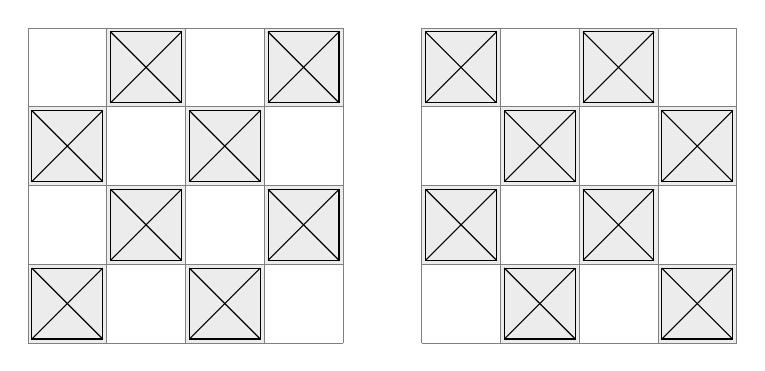
\begin{tikzpicture}
                \foreach \x/\y in {0/0,0/2,1/1,1/3,2/0,2/2,3/1,3/3,5/1,5/3,6/0,6/2,7/1,7/3,8/0,8/2}
                {
                    \fill[fill=gray!15!white] (\x,\y) rectangle (\x+1,\y+1);
                    \draw[black] (\x+.05,\y+.05) rectangle (\x+.95,\y+.95);
                    \draw[black] (\x+.05,\y+.05) -- (\x+.95,\y+.95);
                    \draw[black] (\x+.95,\y+.05) -- (\x+.05,\y+.95);
                }
                \draw[step=1cm,gray,very thin] (0,0) grid (4,4);
                \draw[step=1cm,gray,very thin] (5,0) grid (9,4);
            \end{tikzpicture}
            \caption{Even and Odd tile selection}
            \label{fig:even_odd_chessboard}
        \end{figure}

    % paragraph even_odd (end)

    \paragraph{Singleton Move} % (fold)
    \label{par:singleton}

        La mossa prevede una selezione massimale random di \emph{tiles} e un loro ricombinamento con eventuale rotazione. Ad ogni selezione di una tile, verranno rese inagibili alcune coordinate adiacenti a tale tile: questo consentirà di calcolare agevolmente il $\Delta$-costo. Si veda più in dettaglio la descrizione della mossa per alcune osservazioni sulla massimalità della selezione e sulla gestione di un intorno esponenziale.

    
    % paragraph singleton (end)

    \paragraph{L Move} % (fold)
    \label{par:l}

        La mossa prevede la selezione di cluster di tile che formino una ``L'' con orientamento qualsiasi (si veda la figura \ref{fig:Lmove}). Anche in questo caso viene selezionato un numero arbitrario di cluster, che viene ricombinato in una mossa.

        \begin{figure}[H]
            \centering
            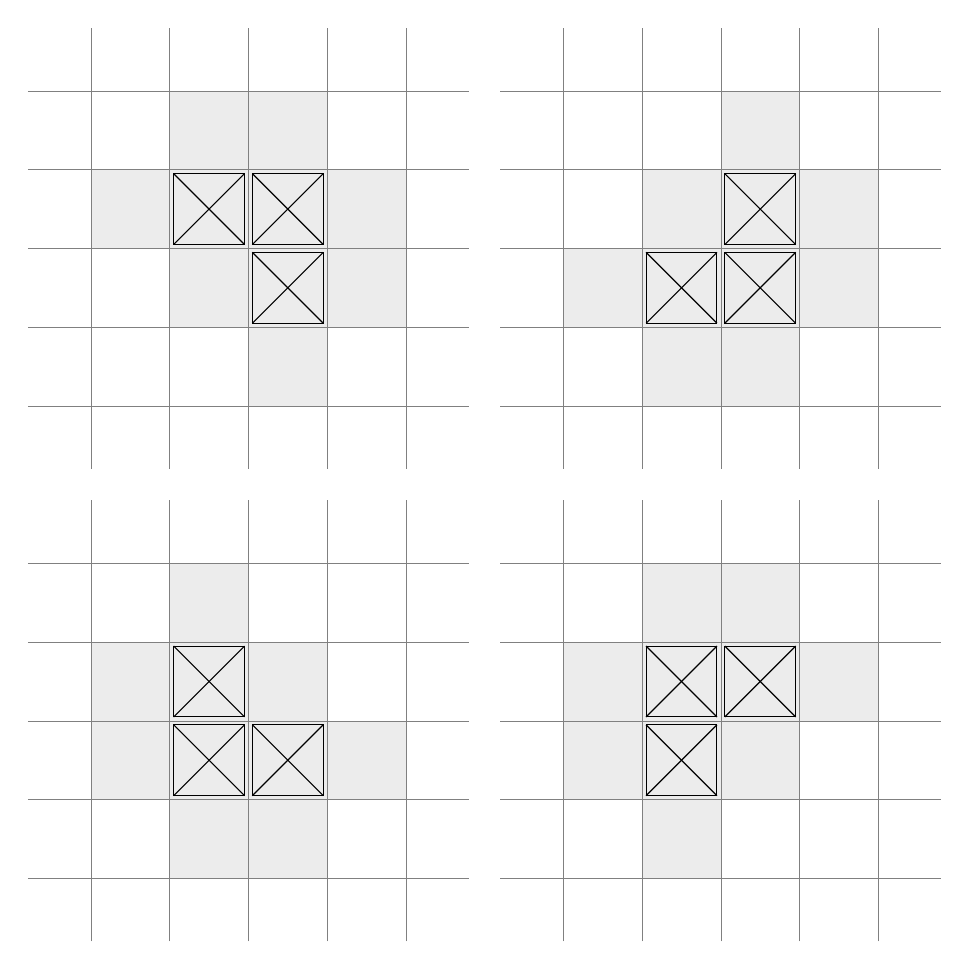
\begin{tikzpicture}
                \foreach \x/\y in {2/2,2/3,3/2,2/4,4/2,3/3,1/2,1/3,2/1,3/1,8/2,8/3,9/3,7/2,7/3,8/4,9/4,9/2,10/3,8/1,3/9,2/9,3/8,2/8,1/9,3/7,3/10,2/10,4/9,4/8,9/9,9/8,8/8,8/9,9/10,7/8,10/9,10/8,9/7,8/7}
                {
                    \fill[fill=gray!15!white] (\x,\y) rectangle (\x+1,\y+1);
                }
                \foreach \x/\y in {2/2,2/3,3/2,8/2,8/3,9/3,3/9,2/9,3/8,9/9,9/8,8/8}
                {
                    \draw[black] (\x+.05,\y+.05) rectangle (\x+.95,\y+.95);
                    \draw[black] (\x+.05,\y+.05) -- (\x+.95,\y+.95);
                    \draw[black] (\x+.95,\y+.05) -- (\x+.05,\y+.95);
                }
                \draw[step=1cm,gray,very thin] (6.2,6.2) grid (11.8,11.8);
                \draw[step=1cm,gray,very thin] (.2,6.2) grid (5.8,11.8);
                \draw[step=1cm,gray,very thin] (.2,.2) grid (5.8,5.8);
                \draw[step=1cm,gray,very thin] (6.2,0.2) grid (11.8,5.8);
            \end{tikzpicture}
            \caption{L Selections}
            \label{fig:Lmove}
        \end{figure}
    
    % paragraph l (end)

    \paragraph{Three--Tile Move} % (fold)
    \label{par:three_tile_move}

        La mossa prevede la selezione di sequenze di tre tile consecutive (orizzontalmente o verticalmente). Come per i casi precedenti, vengono selezionate un numero arbitrario di sequenze e ricombinate con eventuale rotazione.
    
    % paragraph three_tile_move (end)

    Per ogni mossa si è scelto di dividere il processo di \emph{selezione} (delle coordinate) dal processo di \emph{ricombinamento} (delle tiles o dei cluster di tiles). La selezione è fatta nello \textbf{stato} di gioco, mentre la permutazione è parte integrante della mossa. Questo ci ha permesso di ottenere alcuni vantaggi:
    \begin{itemize}
        \item[--] la selezione delle tessere di gioco da muovere può essere fatta con minor frequenza: soprattutto con le mosse random, è possibile mantenere le stesse coordinate per un certo numero di iterazioni, e solo infine rigenerarle;
        \item[--] è possibile applicare l'\emph{Hungarian Algorithm} per il calcolo della \emph{Best Move}, in modo da poter analizzare un intorno esponenziale in tempo polinomiale (si veda per esempio la discussione della BestMove nella sezione della SingletonMove);
        \item[--] non richiediamo che il processo di selezione sia \emph{unbiased} (tranne per la SingletonMove), potendo così sfruttare algoritmi più efficienti.
    \end{itemize}
    
% section overview (end)